\chapter{Viewing library}
\label{cha:Viewing library}

This chapter will present some visualization libraries which could be used to
generate and interact with the components diagram. The comparison between those
libraries is based on the features we want to offer to the KlugHDL user (see
chapter \ref{sec:Goal}). In order to compare those viewing libraries, we end by
discussing the evaluation of all the libraries mentioned.

For the presentation of each of those libraries for graph visualization, we would
use the same graph shown in figure \ref{fig:graph-base-model}.

\begin{figure}[H]
  \centering
  \fbox{
    \digraph[scale=0.5]{GraphBaseModel}{
      node [shape=record];
      graph [rankdir=LR,
      ranksep="1",
      nodesep="1"];
      AndGate [label="{{<a>io.a : Bool|<b>io.b : Bool}|AndGate|{<c>io.c : Bool}}"];
      OrGate [label="{{<a>io.a : Bool|<b>io.b : Bool}|OrGate|{<c>io.c : Bool}}"];
      Input [label="{Input|{<a>io.a : Bool|<b>io.b : Bool}}"];
      Output [label="{{<c>io.c : Bool}|Output}"];
      Input:a -> AndGate:a;
      Input:b -> AndGate:b;
      Input:a -> OrGate:a;
      Input:b -> OrGate:b;
      OrGate:c -> Output:c;
      AndGate:c -> Output:c;
    }
  }
  \caption[Graph model for the viewing library comparison]{The graph we will use
    in order to compare several viewing libraries. This model includes two
    logical components : a AND and a OR gate and two nodes which are
    representing the input and output of the parent component.}
  \label{fig:graph-base-model}
\end{figure}

\section{GraphStream}
\label{sec:GraphStream}

GraphStream is a Java library used for the modeling and analysis of dynamic
graphs\cite{graphstream}. The goal of the library is to provide a way to
represent graphs and work on it\cite{graphstream}. GraphStream is an active
project hosted by the University of Le Havre in France.

\subsection{Implementation of the base graph model}
\label{sub:Implementation}

The figure \ref{fig:base-graph-model-graphstream} shows the base graph model
realised with the GraphStream library.

\begin{figure}[H]
  \centering
  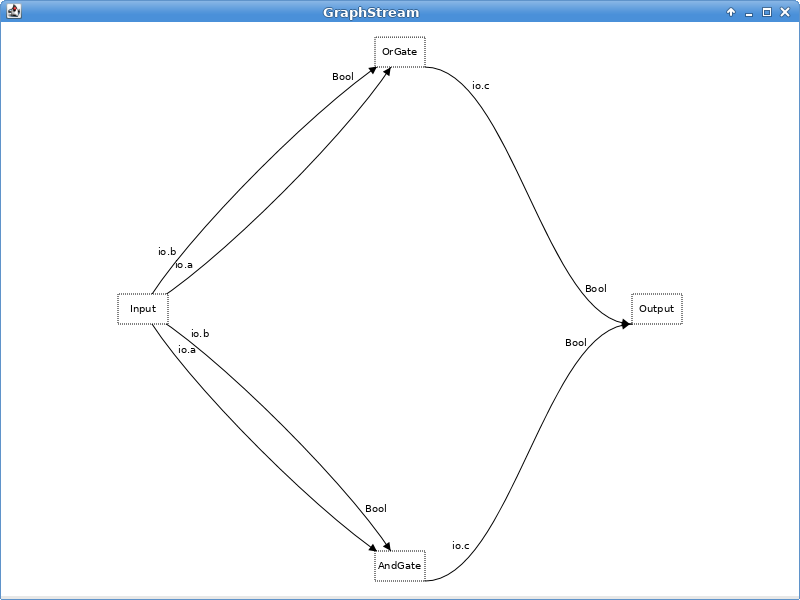
\includegraphics[width=0.8\textwidth]{img/graphstream-base-model-example}
  \caption{The base graph model rendering using GraphStream}
  \label{fig:base-graph-model-graphstream}
\end{figure}

GraphStream allows us to simply create a graph (or a multigraph) in Java like in
listing \ref{lst:graphstream-example}.

\begin{listing}[H]
  \centering
  \begin{javacode}
  Graph graph = new SingleGraph("Example");
  graph.addNode("A" );
  graph.addNode("B" );
  graph.addNode("C" );
  graph.addEdge("AB", "A", "B");
  graph.addEdge("BC", "B", "C");
  graph.addEdge("CA", "C", "A");
  \end{javacode}
  \caption[A simple graph modelisation using GraphStream]{Modeling of a
    simple graph using the GraphStream library}
  \label{lst:graphstream-example}
\end{listing}

\subsection{Remarks}
\label{sub:Remarks}

With GraphStream, there is no way to control some visual features which are very
interesting for hardware component visualization : the splines of the edges and
the anchor position on the node. There is no way to have a node with sub-node
like in the base graph model in figure \ref{fig:graph-base-model}.

An additional special case is the label on the edges. With GraphStream, we could
add some labels on the edges like in listings \ref{lst:graphstream-edge-label},
but we can't add multiple ones. To add multiple labels we need to use sprites like
in listing \ref{lst:graphstream-edge-sprite}.

\begin{listing}[H]
  \centering
  \begin{javacode}
  Graph graph = new MultiGraph("Edges label example");
  graph.addAttribute("ui.quality");
  graph.addAttribute("ui.antialias");
  
  graph.addNode("A");
  graph.addNode("B");
  Edge edge = graph.addEdge("AB", "A", "B", true);
  edge.addAttribute("ui.label", "A --> B");
  graph.display(false);
  \end{javacode}
  \caption[Adding a label on an edge with GraphStream]{A complete example on how to
add a label to an edge with the GraphStream library.}
  \label{lst:graphstream-edge-label}
\end{listing}

\begin{listing}[H]
  \centering
  \begin{javacode}
    SpriteManager sman = new SpriteManager(graph);

    // add label 1
    Sprite label1 = sman.addSprite("label1");
    label1.attachToEdge("AB");
    label1.setPosition(0.2, 0, 0);
    label1.addAttribute("ui.label", "Label 1");
    label1.addAttribute("ui.style", "fill-mode:none;");

    // add label 2
    Sprite label2 = sman.addSprite("label2");
    label2.attachToEdge("AB");
    label2.setPosition(0.8, 0, 0);
    label2.addAttribute("ui.label", "Label 2");
    label2.addAttribute("ui.style", "fill-mode:none;");
  \end{javacode}
  \caption[Adding two labels on an edge with GraphStream]{A complete example on how
to add multiples labels to an edge with the GraphStream library. This time, we
have to use sprites.}
  \label{lst:graphstream-edge-sprite}
\end{listing}

\subsection{Conclusion}
\label{sub:Conclusion-gs}

GraphStream owns other features which could be useful to design an application :
\begin{itemize}
\item View integration using Swing
\item Human-Computer interaction with the view
\item A complete CSS interpretation to personalize the nodes and the edges
\end{itemize}

The main problem using GraphStream is that we need to indicate the component
information using label on the edges. The figure
\ref{fig:base-graph-model-graphstream} shows four nodes and six connections, but
if we have a lot more edges between nodes, it would be difficult to see the
type of the inputs and outputs, as shown in figure
\ref{fig:graphstream-lot-of-edges}.

\begin{figure}[H]
  \centering
  \fbox{
    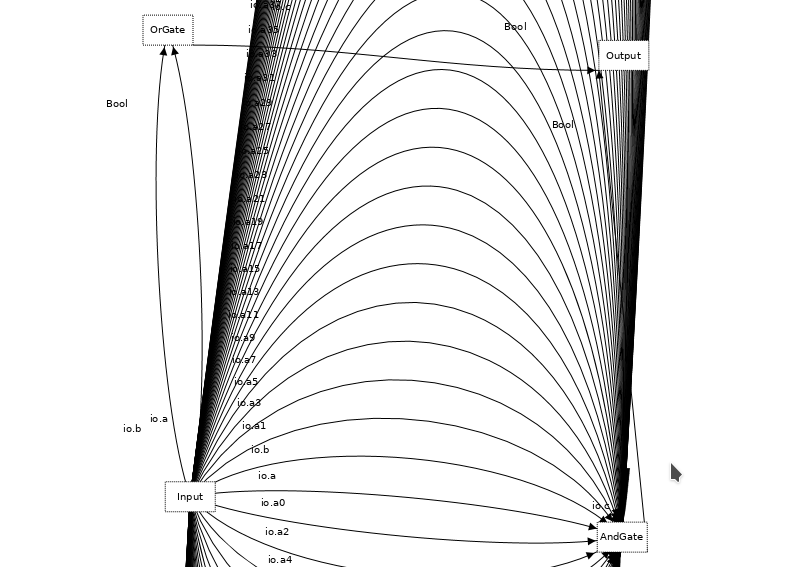
\includegraphics[width=0.8\textwidth]{img/graphstream_lot_of_edges}
  }
  \caption[Label on multiple edges using GraphStream]{}
  \label{fig:graphstream-lot-of-edges}
\end{figure}

In order to overpass those problems, we need to visualize the type in another
form : in the graph \ref{fig:graph-base-model} we had the idea to show the
inputs and outputs as a port of the component. With GraphStream we can't do
it, so we need another library which has this idea of port.

\section{Draw2D}
\label{sec:Draw2D}

Draw2D is a HTML5 and Javascript library for visualization and interaction with
diagrams and graphs\cite{draw2d}. The goal of the library is to provide a way to
represent diagrams and graphs and to manipulate those using the mouse or Javascript
code. Some existing products already use Draw2d for diagrams manipulations :

\begin{itemize}
\item Shape Designer\cite{draw2d}
\item BrainBox\cite{draw2d}
\item Sankey State\cite{draw2d}
\end{itemize}

\subsection{Implementation of the base graph model}
\label{sub:Implementation of the base graph model}

Before implementing directly the basic example of the graph \ref{fig:graph-base-model},
we need to extend the library with a new component for our usage.
In the chapter \ref{sub:Conclusion-gs} we indicate that the GraphStream library
is lacking the idea of port, but Draw2d already has them.

The listing \ref{lst:draw2d-base-graph-model} shows the realisation of the base
graph model example. Note that the object \textbf{ComponentShape} and the
functions \textbf{ComponentShape.addPort()}, \textbf{newConnection()} and
\textbf{createConnection()} are not part of the Draw2d library, it's an
extension added for this project.

The code in the listing \ref{lst:draw2d-base-graph-model} is producing the HTML page shown in
figure \ref{fig:base-graph-model-html-draw2d}.

\begin{listing}[H]
  \centering
  \begin{jscode}
    var canvas = new draw2d.Canvas("gfx_holder1");

    var andGate = new ComponentShape();
    var orGate = new ComponentShape();
    var input = new ComponentShape();
    var output = new ComponentShape();

    canvas.installEditPolicy(new draw2d.policy.connection.DragConnectionCreatePolicy({
      createConnection: createConnection
    }));

    andGate.setName("AndGate");
    orGate.setName("OrGate");
    input.setName("Input");
    output.setName("Output");

    andGate.addPort("io.a", "input");
    andGate.addPort("io.b", "input");
    andGate.addPort("io.c", "output");

    orGate.addPort("io.a", "input");
    orGate.addPort("io.b", "input");
    orGate.addPort("io.c", "output");

    input.addPort("io.a", "output");
    input.addPort("io.b", "output");

    output.addPort("io.c", "input");

    canvas.add(input);
    canvas.add(output);
    canvas.add(andGate);
    canvas.add(orGate);

    canvas.add(newConnection(input.getPort("io.a"), andGate.getPort("io.a")));
    canvas.add(newConnection(input.getPort("io.b"), andGate.getPort("io.b")));
    canvas.add(newConnection(input.getPort("io.a"), orGate.getPort("io.a")));
    canvas.add(newConnection(input.getPort("io.b"), orGate.getPort("io.b")));
    canvas.add(newConnection(andGate.getPort("io.c"), output.getPort("io.c")));
    canvas.add(newConnection(orGate.getPort("io.c"), output.getPort("io.c")));
  \end{jscode}

  \caption[Base graph modeling implementation using the Draw2D library]{The necessary code to produce the base graph model with the Draw2d library.
    The object \textbf{ComponentShape} and the functions \textbf{addPort()},
    \textbf{newConnection()} and \textbf{createConnection()} are not part of the
    Draw2d library, it's an extension added for this project.}
  \label{lst:draw2d-base-graph-model}
\end{listing}


\begin{figure}[H]
  \centering
  \fbox{
    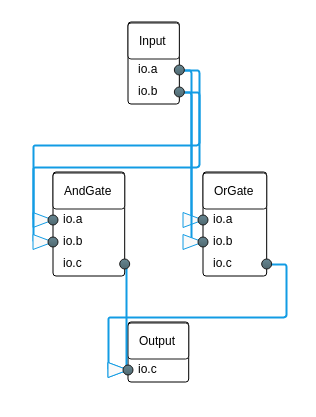
\includegraphics[width=0.3\textwidth]{img/draw2d-base-model-example}
  }
  \caption[Render of the base graph model using the Draw2D library]{Rendering of
    the base graph model diagram from figure \ref{fig:graph-base-model} using
    the Draw2D library}
  \label{fig:base-graph-model-html-draw2d}
\end{figure}

\section{Graph layout}
\label{sec:graph-layout}

A feature that Draw2D doens't own is the layout of the diagram. If we did not
say anything about the position of the node, Draw2D simply overlaps all the nodes
 as illustrated in figure \ref{fig:draw2d_overlapping}.

\begin{figure}[H]
  \centering
  \fbox{
    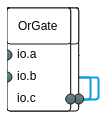
\includegraphics{img/overlap_draw2d}
  }
  \caption[Overlapping of nodes by Draw2D]{When we don't specify the
    nodes positions with Draw2D, the engine just overlaps all the nodes.}
  \label{fig:draw2d_overlapping}
\end{figure}

In order to produce a visualisable diagram, we need to layout ourself the
diagram. We need to mention that the layout algorithm is a NP-Hard problem in
computing theory\cite{Tamassia:2007:HGD:1202383} and for our graph, we have some
specialties :

\begin{itemize}
\item The graph could be cyclic
\item The graph is oriented
\item Nodes own ports, so we need to layout the edges on a specific part of the graph.
\end{itemize}

The first two specialties aren't a big deal, but the last one is quite
problematic. It involves a special layout algorithm which takes care of the ports
position on the nodes. Otherwise the visual result could be chaotic like in
figure \ref{fig:multigraph-no-port}, in which we can't see the connections
between some specific ports.

\begin{figure}[H]
  \centering
  \fbox{
    \digraph[scale=0.5]{MultiGraphNoPort}{
      A -> B -> C -> D;
      A -> B -> C;
      A -> B;
      D -> A;
      D -> B;
    }
  }
  \caption[Visualization of a multi-graph without port]{Visualization of a
    multi-graph without port. We can't differentiate the connections between two
  differents ports on the same component.}
  \label{fig:multigraph-no-port}
\end{figure}

In order to solve this drawback, we need to layout the graph ourselves by using a
library. We could also do it ourselves by implementing the algorithm for the kind
of graph we have, but it's too much time-consuming for a project like this.

\section{Conclusion}
\label{sec:viewing-library-conclusion}

GraphStream looks like a really good library for manipulating graphs and visualize
them. The problem is that there is no good way to visualize the ports of the
components so we have to labelize the connections and it looks ugly (figure
\ref{fig:graphstream-lot-of-edges}). Then we have to find a library which allows
this idea of ports. We found them with Draw2D and chose it for the project. The
disadvantage of using this library is that we can't layout easily the graph by
ourselves.

%%% Local Variables:
%%% mode: latex
%%% TeX-master: "../report"
%%% End: